\section{What device noise does to the energy}
\label{sec:noise}

On a noisy device the circuit prepares a mixed state $\rho$ instead of $\ket{\psi(\theta)}$, and
the measured energy is $\operatorname{Tr}(\rho H)$. This section explains why that energy sits on
a plateau far above $-18$ even at the exact parameters, and why the plateau is nearly a constant
\emph{factor} times the ideal energy. That structure decides which improvements can work.

\begin{prop}[Variational principle for mixed states]\label{prop:mixed}
  For every density matrix $\rho$, $\operatorname{Tr}(\rho H)\ge E_0$.
\end{prop}

\begin{proof}
  Write $\rho=\sum_k p_k\ket{\chi_k}\bra{\chi_k}$ with $p_k\ge0$, $\sum p_k=1$. Each
  $\bra{\chi_k}H\ket{\chi_k}\ge E_0$, and a convex combination of numbers $\ge E_0$ is $\ge E_0$.
\end{proof}

Hence a noisy reading \emph{below} $-18$ cannot come from a physical state; it signals sampling
fluctuation or an over-corrected mitigation, never a better answer.

\begin{prop}[Depolarising noise rescales the energy]\label{prop:depol}
  Let $\mathcal D_p(\rho)=(1-p)\rho+p\,I/2^{n}$. Then $\operatorname{Tr}(\mathcal D_p(\rho)H)=(1-p)\operatorname{Tr}(\rho H)$.
  If each qubit's readout flips independently with probability $q$, every two-qubit Pauli
  expectation is multiplied by $(1-2q)^2$, so the measured energy is $(1-2q)^2\operatorname{Tr}(\rho H)$.
\end{prop}

\begin{proof}
  $\operatorname{Tr}(H)=0$ because every term of $H$ is a non-identity Pauli string, so the
  maximally mixed part contributes nothing. For readout, a $\pm1$ outcome flipped with
  probability $q$ has mean $(1-2q)$ times the true mean, and the two outcomes of a $ZZ$-type term
  flip independently, giving $(1-2q)^2$. The same holds in the $X$ and $Y$ bases, where the
  measurement is a $Z$ measurement after a basis rotation.
\end{proof}

Real device noise is neither global nor uniform, but if it were, the two factors would simply
multiply. Table~\ref{tab:floor} tests that by switching the noise channels of the
\py{FakeGuadalupeV2} model on one at a time, at the exact parameters, with \VNoiseShots{} shots
per basis.

\begin{table}[H]
  \centering
  % Generated by `uv run python -m docsgen`; do not edit.
\begin{tabular}{lccccc}
\toprule
ansatz & noise-free & readout only & gate + $T_1/T_2$ only & full & $E_0\, r_{\mathrm{ro}}\, r_{\mathrm{g}}$ \\
\midrule
HVA & \VFloorHvaIdeal & \VFloorHvaReadout & \VFloorHvaGate & \VFloorHvaFull & \VKeepHvaProduct \\
RVB & \VFloorRvbIdeal & \VFloorRvbReadout & \VFloorRvbGate & \VFloorRvbFull & \VKeepRvbProduct \\
\bottomrule
\end{tabular}

  \caption{Energy at the exact parameters (all zero) on \py{FakeGuadalupeV2}, transpiled to
    \VCxHva{} CX. Readout error alone retains $r_{\mathrm{ro}}=\VKeepHvaReadout$ of the energy;
    gate and $T_1/T_2$ errors alone retain $r_{\mathrm g}=\VKeepHvaGate$ (HVA). The last
    column multiplies the two factors and nearly matches the full model.}
  \label{tab:floor}
\end{table}

\begin{figure}[H]
  \centering
  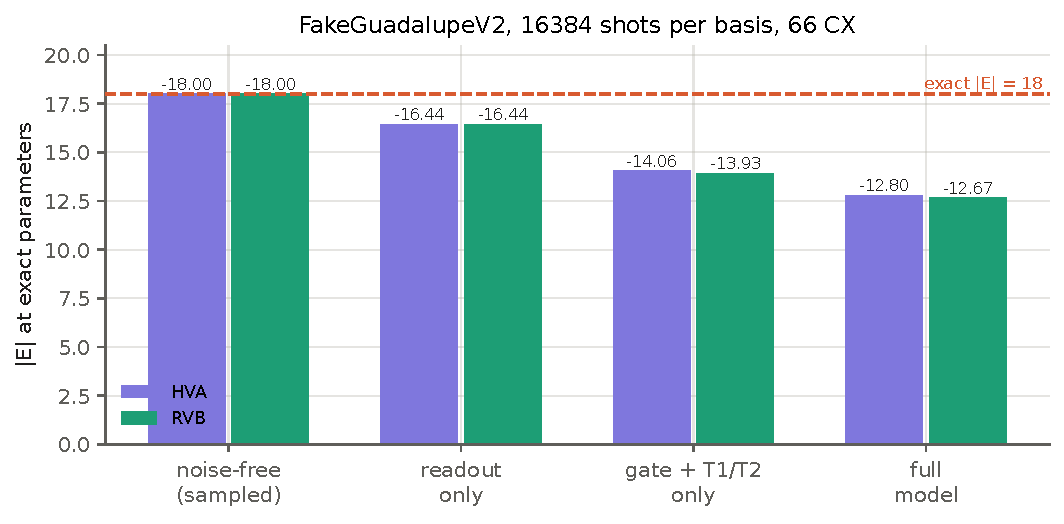
\includegraphics[width=0.75\linewidth]{noise_floor}
  \caption{The same data. The noisy energy is not a convergence failure: the exact optimum
    itself reads \VFloorHvaFull{} (HVA) under the full model. The near-multiplicative structure
    (readout $\times$ gate $\approx$ full) is what makes rescaling-type mitigation promising.}
  \label{fig:floor}
\end{figure}

\begin{prop}[Zero shot noise at the exact optimum]\label{prop:zerovar}
  In each of the three measurement bases, every shot taken on $\ket{D_{M_1}}$ returns the same
  value $-6$ for that basis's part of $H$. The sampled energy is exactly $-18$ with zero variance,
  for any number of shots.
\end{prop}

\begin{proof}
  Take the $Z$ basis; $X$ and $Y$ are identical because a singlet is anticorrelated along every
  axis. A shot returns $z\in\{\pm1\}^{12}$ with $z_i=-z_{6+i}$ on every dimer
  $\{i,6+i\}\in M_1$. The $ZZ$ part of $H$ evaluates to
  \[
    \sum_{i=0}^{5}z_iz_{6+i}+\sum_{i=0}^{5}\bigl(z_iz_{i+1}+z_{i+1}z_{6+i}\bigr)
    =-6+\sum_{i=0}^{5}\bigl(z_iz_{i+1}-z_{i+1}z_{i}\bigr)=-6,
  \]
  grouping the 12 unmatched bonds by triangle: in $\tau_i$, the hexagon bond and the second spoke
  share site $i+1$ and see $z_i$ and $z_{6+i}=-z_i$ respectively.
\end{proof}

\Cref{prop:zerovar} has a practical side. The real spread of sampled energies falls towards
zero as the parameters approach the optimum: \VSpreadLowReal{} at the start point
$(\phi,\gamma)=(\pi/4,\pi/4)$ with 1024 shots, \VSpreadLowZero{} at the optimum. The primitive's
reported standard error is a state-independent bound (\cref{sec:m0}) and does not show this.
Noise-free sampled runs therefore become \emph{easier} as they converge; with device noise the
mixed state breaks the cancellation and the shot noise stays.

\subsection*{Exercises}

\begin{exer}
  Using \cref{prop:depol} and Table~\ref{tab:floor}, estimate the uniform readout flip
  probability $q$ that would explain the readout-only energy of HVA.
\end{exer}
\begin{sol}
  $(1-2q)^2=\VKeepHvaReadout$, so $1-2q\approx0.956$ and $q\approx2.2\,\%$, a typical readout
  error for that device generation.
\end{sol}

\begin{exer}
  Why does \cref{prop:zerovar} not contradict the fact that the individual terms $X_iX_j$ on
  unmatched bonds have nonzero variance on $\ket{D_{M_1}}$?
\end{exer}
\begin{sol}
  The terms are random individually, but within a triangle the two unmatched terms are
  perfectly anticorrelated, shot by shot, so their sum is deterministic. Variance of a sum
  includes covariances, which cancel the individual variances here.
\end{sol}
